\chapter*{Annexe B}
\addcontentsline{toc}{chapter}{Annexe B}

%recommencer la numérotation des section à "1"
\setcounter{section}{0}

Dans cette annexe, nous présentons les tâches préventives à effectuer pour le système de messages aéronautiques STANOS.


\section*{Ce qu’il savoir faire sur le STANOS}
\begin{itemize}
\item Arrêt et Démarrage d’un PC client /serveur et de l’application BIA (Bureau d’information aéronautique)  et Distribution.\\
\item Dépannage d’une imprimante (réinstallation, bourrage, changement de ruban, …). \\
\item Basculement Onduleur sur batterie et retour sur Secteur.\\
\item Méthode de réclamation Frame Relay.\\
\item Test de continuité d’une ligne. \\
\item Contrôle de la ligne FR.\\
\end{itemize}
\section*{Tâches quotidiennes}
\begin{itemize}
\item Vérifier l’état général. \\
\item Vérifier la disponibilité des équipements: il s’agit d’une vérification visuelle dans l’application « Gestion des équipements STANOS ».
\begin{figure}[!h]
\begin{center}
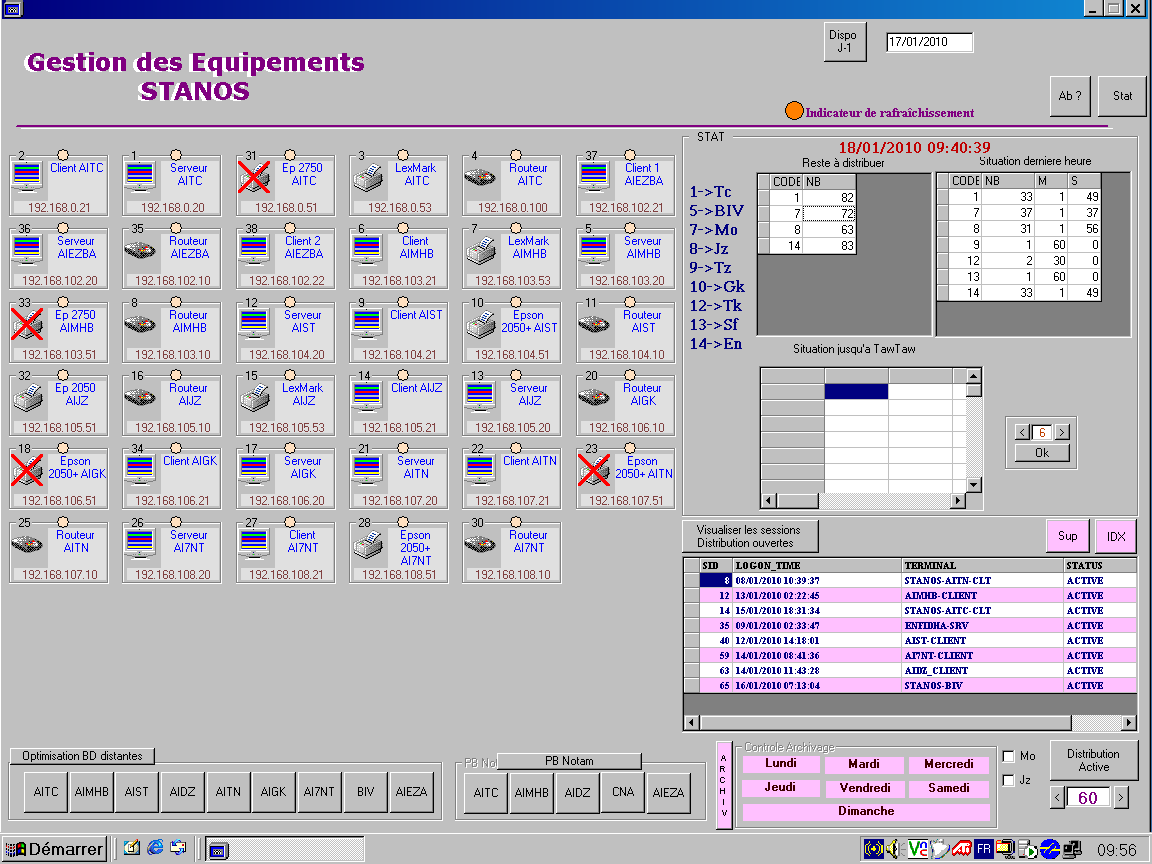
\includegraphics[width=10cm,height=7cm]{annexes/Gestion_des__quipements_STANOS.png}
\end{center}
%légende de l'image
\caption{Capture de l'application de gestion des équipements STANOS}
\end{figure}
\item Archivage de la base centrale sur le PC de supervision.\\
\item Optimisation de la distribution des messages par lancement d’une procédure de réindexassions et d’analyse des bases de données centrale et vérification des fichiers « log » qui contiennent un compte rendu de la dite procédure.\\
\item Archiver les données centrales + BIV sur une bande.
\item Vérifier le déroulement des Backups: archivage des données de chaque base  distante.\\
\item Vérifier la distribution des messages: taux de messages par minutes.\\
\item Vérifier l’état général des onduleurs.\\
\item Remplir la fiche GMAO.\\
\begin{figure}[!h]
\begin{center}
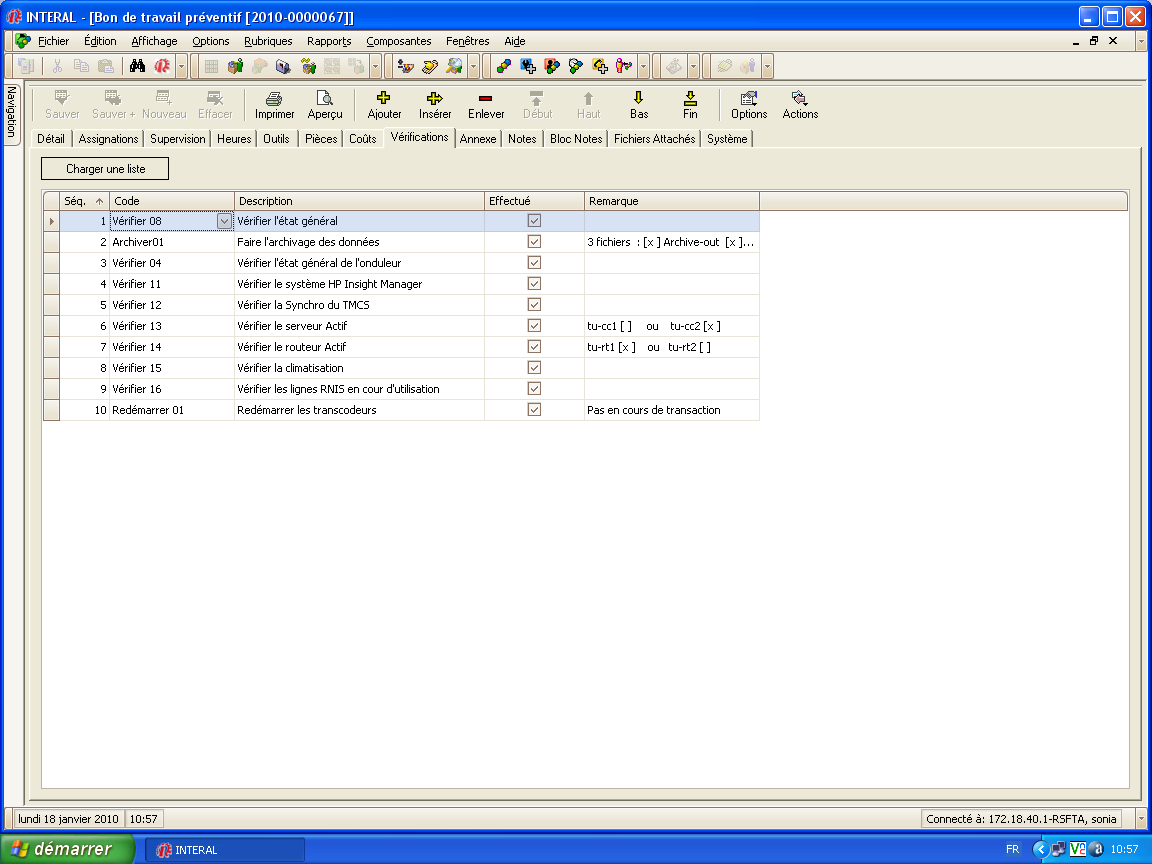
\includegraphics[width=10cm,height=7cm]{annexes/GMAO.png}
\end{center}
%légende de l'image
\caption{Capture de l'opération de remplissage de la fiche GMAO}
\end{figure}
\end{itemize}
\section*{Taches hebdomadaires}
\begin{itemize}
\item Optimisation de la distribution des messages par le lancement d’une procédure de réindexassions et d’analyse des bases de données distantes et vérification des fichiers « log » qui contiennent un compte rendu de la dite procédure.\\
\item Vérifier de l’espace libre disponible des disques système avec la commande \#df –k. (l’espace libre ne doit pas être inférieur à 20\% de l’espace total). \\
\item Synchronisation horaire entre les terminaux et la centrale (Manuellement).\\
\end{itemize}
\section*{Tâches mensuelles}
\begin{itemize}
\item Test des onduleurs: La maintenance de l’onduleur s’effectue tous les 30 jours, en coupant le secteur afin de vérifier son bon fonctionnement et pour tester la capacité des batteries. \\
\item Compactages des bases de données du module réception :
\begin{itemize}
\item Rendre esclave.\\
\item Arrêter l’application. \\
\item Désactiver le réseau. \\
\item Compacter la première base.\\
\item Redémarrer l’application.\\
\item Même procédure pour la deuxième base.\\
\end{itemize}
\end{itemize}

\begin{center}
\textbf{Remarque !}

\textit{Chaque tâche est planifiée dans le système GMAO (Gestion de maintenance assistée par ordinateur) et l'ingénieur est appelé à remplir le bon fonctionnement de la tâche réalisée.
 La validation est faite par le chef service.
}
\end{center}

\section*{Maintenances curatives}

\begin{table}[!h]
\begin{center}
\begin{tabular}{|p{8cm}|p{8cm}|}
  \hline
     \textbf{Problèmes} & \textbf{Solutions} \\
   \hline
   Pas de réception de trafic à SIDI AHMED &  -Remise à zéro du transcodeur de SIDI AHMED (coté CCR) -Demander aux techniciens de remettre à zéro le  transcodeur (coté SIDI AHMED) -Redémarrer le transcodeur de SIDI AHMED       -Relancer l’application ‘’IAT’’ -Vérifier que le test du transcodeur est bien reçu  \\ \hline
Panne de l’ATIS d’ENFIDHA & Contacter le technicien d’ENFIDHA ; problème reconnu par le fournisseur. \\ \hline
Faute de manipulation d’un onduleur au centre médical  & Déplacement sur place et réorganisation du branchement des équipements sur l’onduleur \\ \hline
Au cours du test de l’onduleur de STANOS on remarquer que l’autonomie batterie de cet onduleur est très faible. & Remplacement urgent par un autre onduleur plus performant. \\ \hline

  \end{tabular}
\end{center}
\caption{Tableau récapitulatif des problèmes possibles et leurs solutions}
\end{table}